\documentclass[border=10pt,crop=true]{standalone}
\usepackage{tikz}

% 坐标用「单位 = 10 V」：13 V → 1.3
\def\OpSat{1.3}
\def\OpKnee{0.13}

\begin{document}
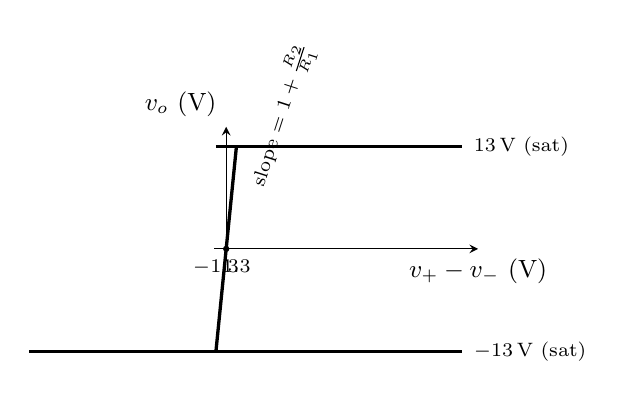
\begin{tikzpicture}[>=stealth, font=\small]
  \draw[->] (-0.15, 0) -- (3.2, 0) node[below] {$v_+-v_-$ (V)};
  \draw[->] (0, -0.15) -- (0, 1.55) node[above left] {$v_o$ (V)};

  \draw[very thick] (-\OpKnee, -\OpSat) -- (\OpKnee, \OpSat);
  \node[font=\scriptsize, rotate=72, anchor=west] at (0.38, 0.68)
    {slope $=1+\frac{R_2}{R_1}$};

  \draw[very thick] (-\OpKnee, \OpSat) -- (3.0, \OpSat);
  \draw[very thick] (-\OpKnee, -\OpSat) -- (3.0, -\OpSat);
  \draw[very thick] (-\OpKnee, -\OpSat) -- (-2.5, -\OpSat);

  \node[font=\scriptsize, anchor=west] at (3.02, \OpSat) {$13$\,V (sat)};
  \node[font=\scriptsize, anchor=west] at (3.02, -\OpSat) {$-13$\,V (sat)};

  \node[font=\scriptsize, anchor=north] at (\OpKnee, -0.02) {$1.3$};
  \node[font=\scriptsize, anchor=north] at (-\OpKnee, -0.02) {$-1.3$};

  \fill (0, 0) circle (0.04);
\end{tikzpicture}
\end{document}
